\documentclass[tikz, border=4pt]{standalone}
\usepackage{tikz}
\usepackage{pgfplots}
\pgfplotsset{compat=1.18}
\begin{document}
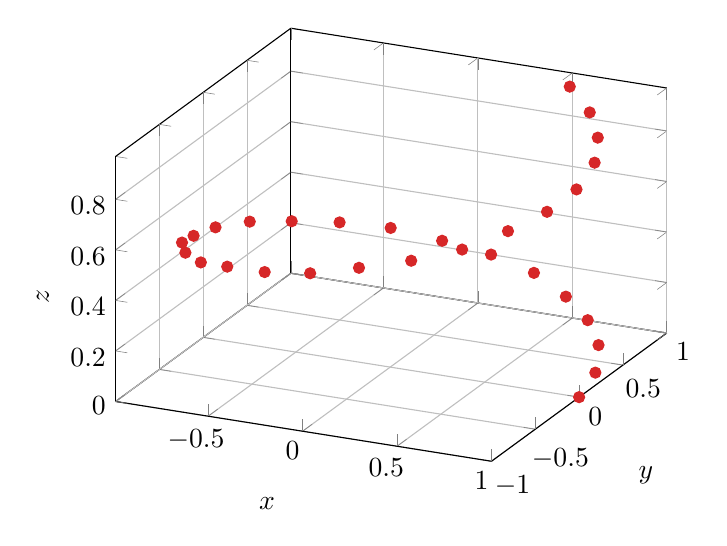
\begin{tikzpicture}[x=1cm, y=1cm]
  \definecolor{tdc1}{HTML}{D62728}

  \begin{axis}[
    at={(0cm,-5.5cm)},
    anchor=south west,
    scale only axis,
    width=7cm,
    height=5.5cm,
    xmin=-0.99,
    xmax=1,
    ymin=-1,
    ymax=1,
    zmin=0,
    zmax=0.97,
    view={25}{30},
    xtick={-0.5,0,0.5,1},
    ytick={-1,-0.5,0,0.5,1},
    ztick={0,0.2,0.4,0.6,0.8},
    grid=major,
    xlabel={$x$},
    ylabel={$y$},
    zlabel={$z$}
  ]
    \addplot3[color=tdc1, only marks, mark=*, forget plot] coordinates {(1,0,0) (0.97,0.25,0.03) (0.88,0.48,0.07) (0.73,0.68,0.1) (0.54,0.84,0.13) (0.32,0.95,0.17) (0.07,1,0.2) (-0.18,0.98,0.23) (-0.42,0.91,0.27) (-0.63,0.78,0.3) (-0.8,0.6,0.33) (-0.92,0.38,0.37) (-0.99,0.14,0.4) (-0.99,-0.11,0.43) (-0.94,-0.35,0.47) (-0.82,-0.57,0.5) (-0.65,-0.76,0.53) (-0.45,-0.89,0.57) (-0.21,-0.98,0.6) (0.04,-1,0.63) (0.28,-0.96,0.67) (0.51,-0.86,0.7) (0.71,-0.71,0.73) (0.86,-0.51,0.77) (0.96,-0.28,0.8) (1,-0.03,0.83) (0.98,0.22,0.87) (0.89,0.45,0.9) (0.75,0.66,0.93) (0.57,0.82,0.97)};
  \end{axis}
\end{tikzpicture}
\end{document}
